\chapter{背景}
\label{background}

本章では,本研究の背景について概説する.

本研究における惑星規模の分散システムを定義し,惑星規模の分散システムの基盤技術であるP2Pについて概説する.
加えて,本研究で対象とする試験環境の定義と惑星規模の分散システムに必要な試験環境について述べる.
最後に,本研究の提案手法で用いるコンテナオーケストレーションシステムとOpenVPNについて概説する.

\section{惑星規模の分散システム}
\label{bg:definition}

本節では,本研究が対象とする惑星規模の分散システムを定義する.
惑星規模の分散システムについて概説する前に,分散システムについて詳細を述べ,違いを明らかにした上で本研究における惑星規模の分散システムを定義する.

\subsection{分散システム}
\label{bg:definition:distributed-system}

分散システムとは,複数の構成要素が協調動作することによって成り立つシステムを指す.
各構成要素は独立して異なる役割を持っており,それらが組み合わさり互いに協調動作することによってシステム全体が動作する.
本研究で使用するKubernetesも,コンテナオーケストレーションに必要な機能を構成要素毎に分割した分散システムである.
Kubernetesに関する説明は~\ref{background:container-orchestration-system:kubernetes}章で詳しく行う.
分散システムは複雑に思われるが,機能が細分化され各構成要素の役割が明確化されるメリットがある.
機能同士の依存関係が希薄になるため細かい粒度での試験が可能となり,障害時の原因特定も行いやすい.
チーム開発において開発者同士で担当範囲が重複する可能性も下がるため,開発スピードが向上するというメリットもある.

\begin{figure}[htbp]
\begin{center}
    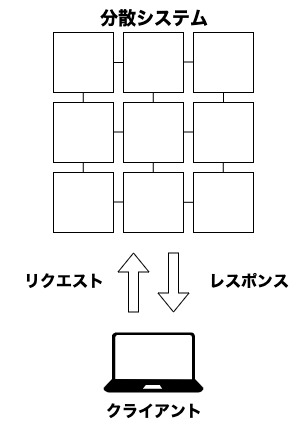
\includegraphics[width=0.4\textwidth]{./figures/distributed-system.jpg}
    \caption{分散システム}
\end{center}
\end{figure}

\subsection{惑星規模の分散システム}
\label{bg:definition:planetary-scale-distributed-system}

本研究における惑星規模の分散システムとは,分散システムの中でも世界中に地理的に分散したコンピュータが協調動作することによって成り立つシステムを指す.
近年注目を集めているブロックチェーンや2000年代初頭に登場したWinnyといったサービスが,惑星規模の分散システムの一例である.
惑星規模の分散システムを支える技術や例についての概説は~\ref{bg:planetary-scale-distributed-system}にて行う.
惑星規模の分散システムでは,システムを構成するコンピュータが地理的に分散していることから,開発者はネットワークでの通信の遅延を考慮する必要がある.

\section{惑星規模の分散システムにおける使用技術と参考例}
\label{bg:planetary-scale-distributed-system}

本節では,~\ref{bg:definition:planetary-scale-distributed-system}章で概説した惑星規模の分散システムを支える技術とサービス例について概説する.
惑星規模の分散システムの基盤技術として,P2Pがあげられる.
P2Pシステムは中央集権的なサーバを必要としないクライアントサーバモデルとは対照的なシステムモデルである.
P2Pについて概説したのち,P2Pシステムを採用するサービスとして, Winny, Gnutella, Bitcoinを紹介する.

\subsection{P2P}
\label{bg:planetary-scale-distributed-system:p2p}

P2Pは``Peer to Peer''の略記である.
P2Pは,クライアントサーバモデルのシステムのように中央集権的な役割を担うサーバを必要とせず,コンピュータ同士が対等な関係を築く主従関係のないシステムモデルである.
またはそれを実現する技術を指す.

クライアントサーバモデルでは,通信においてサーバとクライアントで常に一対一の関係性が成り立つ.
また,システム内では処理や情報を要求するクライアントと要求に対し応答するサーバで明確な役割分担がある.
サーバはクライアントから要求が送られてきた際は,特定の処理を行いクライアントに対し情報を返すが,それ以外では待機状態となる.
対してクライアントは,情報を要求したり変更してもらう必要が生じた際のみサーバと通信を行う.
よってクライアントサーバモデルにおける通信は,基本的にクライアントが起点となって行われる.

P2Pでは各コンピュータが互いに対等な関係性を築くため,クライアントサーバモデルのような明確な役割分担がシステム上ない.
P2Pでは,各コンピュータが状況に応じてサーバとクライアントの役割を担う.
各コンピュータが臨機応変にサーバとして要求に応答し,クライアントとして処理や情報を要求する動的システムが特徴としてあげられる.

クライアントサーバモデルでは,要求する側をクライアント,対して要求に応じる側をサーバと呼んでいる.
P2Pでは前述した通り各コンピュータは動的に役割を変化させ,サーバとしてもクライアントとしても動作することからサーバントと呼ばれる.
または単にノードと呼ばれることもある.

\subsubsection{P2Pの特徴}

P2Pでは各コンピュータがサーバにもクライアントにも成り得るため,クライアントサーバモデルとは内部の実装も異なる.

第一に,データを保持する中央集権的なサーバが存在しないためアプリケーション上で必要になるデータは各コンピュータが保持する.
アプリケーションの実装方式によっても異なるが,各コンピュータがデータを分割して保持する場合もあれば全てのコンピュータが同じデータを保持する場合もある.
例えばファイル共有システムであるWinnyでは,各コンピュータの保持しているデータは異なるため,
データを参照する際はどのコンピュータが目的のデータを保持しているか検索し,対象となるコンピュータを決定してから通信を行う必要がある.
また,ブロックチェーンでは各コンピュータが全てのデータを保持しており(全てのデータを持たない場合もある),データを相互に検証し合うことによってデータの改竄耐性を向上させ,堅牢性を担保している.

次に,システムのメインプログラムを各コンピュータが保持し動作させなければいけない点でもクライアントサーバモデルとは異なる.
クライアントサーバモデルでは,システムのメインプログラムの実行はサーバの役割であるため,サーバのみがシステムのメインプログラムを保持しておけば良い.
対して,各コンピュータが状況に応じて役割を変えるP2Pではシステムのメインプログラムを各々で保持する必要性がある.
クライアントとして他のコンピュータが保持しているデータを参照したり,情報を要求してきたコンピュータに対して応答をしなければならないからである.

\subsubsection{P2Pのメリット}

本節では,P2Pのメリットについて概説する.
P2Pシステムの利点としては,拡張性(スケーラビリティ)・耐障害性があげられる.

第一に拡張性に関しては,クライアントサーバモデルの場合,利用者が増大するとシステムの中心であるサーバへアクセスが集中し,サーバやその周辺のネットワークへの負荷が高くなり,システム的な弱点になる.
システム運用者は拡張性を高めるため,ネットワーク機器のスペックをあげたり,負荷が増大した際に自動でサーバの数を増やすオートスケーリングなどの対策を取らなければならない.
それに対してP2Pの場合,コンピュータ同士は相互に通信を行うためアクセスは分散されやすくなる.
その点でP2Pは拡張性に長けている.

次に耐障害性である.
クライアントサーバモデルの場合,何らかの原因でサーバが落ちるとシステム自体が停止してしまいサーバが構造上の単一障害点となる.
しかし,P2Pではあるコンピュータが停止した場合でも,正常なコンピュータ同士で新たなネットワークを形成することで滞りなくシステムの動作を継続することができる.
構造上の単一障害点が存在しないため,障害性に長けている.

\subsubsection{P2Pのデメリット}

本節では,P2Pのデメリットについて概説する.

第一に情報伝達における遅延があげられる.
P2Pでは接続先のコンピュータが常に決まっていないため,状況に応じて接続先を変更する必要がある.
すなわち,目的の情報を保持しているコンピュータを探し出したり,そもそもネットワーク上で近い距離に他のコンピュータが存在しない場合,情報の取得や送信に遅延が生じてしまう.
全てのコンピュータで同じデータを保持するブロックチェーンのようなシステムにおいては,コンピュータ同士がバケツリレーのようにデータを受け渡さなければならず,端から端までデータを伝えるまでに時間が掛かってしまう問題点がある.

次にシステム全体での管理のしにくさがあげられる.
P2Pシステムでは各コンピュータでアプリケーションを動作させるため,中央集権的なサーバと異なり,管理は各コンピュータ管理者に委ねられることになる.
よって,システムに問題点が見つかり開発者が修正を含んだ更新版を配布した場合でも,実際に動作しているアプリケーションが更新されるかどうかは保証されない.
同様にシステム全体の監視を行うことも困難である.

\subsection{Winny}

Winny~\cite{Winny}はソフトウェアエンジニア金子勇氏が開発し,2002年に発表されたファイル共有ソフトである.
システム上で中央集権的なサーバを保持せず,コンピュータ同士が相互に接続することで実現されるP2Pアプリケーションとして注目を浴びた.
ユーザはコンピュータ内に保持されたファイルを他のコンピュータと共有することができるため,任意のファイルをアップロードしたり,逆に他のコンピュータが保持しているファイルをダウンロードすることができる.
Winnyでは,受信ファイルの送信元や送信ファイルの宛先をユーザが確認することはできず,バックグラウンドでの処理はユーザに見せないよう高い秘匿性が担保されていた.
クライアントサーバモデルのシステムアーキテクチャとは打って変わって出た新しい形のアプリケーションであったが,高い匿名性も起因して,一部のユーザが違法な音楽ファイルや動画ファイル,コンピュータウイルスをWinnyにアップロードしたことで著作権法違反が問われた.
開発者である金子氏にも疑いがかけられ2004年に逮捕,その後画期的な発明であったWinnyも衰退していった.
なお,金子氏は裁判を経て2011年に無罪となった.

\subsection{Gnutella}

Winnyに同じくGnutella~\cite{Gnutella}も中央集権型サーバに依存せず,コンピュータ間の通信のみでファイルの送受信を行うファイル共有アプリケーションである.
ファイルと言えど,Gnutellaでは主に音楽ファイルが共有されていた.
GnutellaはAOL(アメリカ・オンライン)社のチームが開発したものである.
著作権保護の観点から,法的に違法性を問われ公開も開発もすぐに中止されてしまった.
Gnutellaでは,最初のプログラムの起動時には,接続先を自動で認識できないためファイル交換や検索機能は使用できない.
Gnutellaのシステムへ参加したい場合は,メールや掲示板を通して他のGnutellaサーバのIPアドレスとポート番号を教えてもらい,自分のGnutellaサーバへ設定することで他のサーバとの通信を確立できる.
通信確立後は,最初に接続したGnutellaサーバを通して他のサーバとも連携を取ることが可能となり,音楽ファイルの交換や検索を行うことができる.

\subsection{Bitcoin}

Bitcoin~\cite{Bitcoin}は2008年にSatoshi Nakamotoと名乗る人物によって論文にて提唱されたものである.
2009年にはソフトウェアとして公開されており,今では多くのユーザに使用されている上,仮想通貨の先駆けとして他の仮想通貨を生む大きな起点となった.
同時に,2000年代後半に勢いを失っていたP2Pシステムの存在を再度世に知らしめ,開発の促進を促す起爆剤の役割を果たしたと考えられる.
Bitcoinは基盤技術のひとつとしてWinnyやGnutellaと共通するP2Pネットワークを採用している.
参加するコンピュータはそれぞれがシステム上のデータを保持し相互にデータを検証しあうことで,第三者的監視機関を必要とせずにデータの堅牢性を担保することが可能である.

\section{試験環境}
\label{bg:staging}

本節では,本研究で着目する試験環境について概説する.

試験環境とは,システムの試験を行うための環境である.
開発したシステムを公の実稼働環境へ適応する前に,試験環境にて期待する動作を正常に行うか試験する.
試験環境でシステム上の不備を発見した場合,実稼働環境への適応はせずに開発環境にて修正を行う.
対して,試験環境でのシステムの正常な動作を確認できた場合は,実稼働環境への適用作業へ移行する.
開発環境と実稼働環境の間に試験環境を設けることで,システムの予期せぬ不具合を早期に発見できる.

以下,惑星規模の分散システムの試験に必要となる試験環境について概説する.

\subsection{惑星規模の分散システムの試験環境}
\label{bg:staging:planetary-scale-distributed-system}

惑星規模の分散システムは,地理的に分散した構成要素によって成り立つシステムである.
独立した構成要素が互いに協調動作することによってシステム全体が動作している.
分散システムでは,構成要素単位での試験とシステム全体での協調動作の試験が必要である.
なお惑星規模の分散システムの試験においては,システムを構成するコンピュータが地理的に分散していることによるネットワークでの通信の遅延の影響を考慮する必要がある.
通信の遅延を加味した上で分散システムの協調動作が正常に働いていることを確認できれば,公の実稼働環境においても障害発生の可能性が低くなる.
よって,惑星規模の分散システムの試験環境では各コンピュータを地理的に分散させて配置させる必要がある.

惑星規模の分散システムの試験環境としては, PlanetLabやパブリッククラウドサービスの活用, BSafe.networkがあげられる.

PlanetLabは,ネットワークサービスの開発を支援する公の研究ネットワークであり,世界中の717地域1353のサーバをsshを通して利用することができる.
各サーバは仮想マシンを提供しており,研究者に割り当てられる仮想マシンはSliceと呼ばれる.
2003年から指導し,1000人以上の研究者が分散ストレージ,ネットワークマッピング,P2Pシステム,分散ハッシュテーブルなどの新たな技術の開発のためにPlanetLabを利用している.

GCPやAWS, Azureといったパブリッククラウドサービスでは,リージョンと呼ばれるデータセンターの地域を指定することでサーバの地理的な分散配置が可能である.

BSafe.networkは32の大学で構成されるブロックチェーン技術の研究を行うためのネットワークである.
BSafe.networkは政治的かつ経済的に中立的な大学のみで構成される.
研究を行う場合は,世界中の各大学が保有するサーバを用いて実験を行うことができる.

\section{コンテナオーケストレーションシステム}
\label{background:container-orchestration-system}

コンテナオーケストレーションシステムは,コンテナ型仮想環境を統合管理するためのプラットフォームおよびツールを指す.
2010年代半ばから脚光を浴びるようになり,今では世界的に数々のプロジェクトで実稼働環境に適用されている.
サービスの立ち上げや運用過程において必要となる機能が数多く搭載されており,開発者は素早くかつ効率的に開発を進められる.
コンテナはVirtual Machine(以下,VM)のデメリットを考慮して作られており,今後VMの代わりを担う次世代の技術としてより一層注目されていく技術であると考える.

本研究では,コンテナオーケストレーションシステムとしてKubernetesを,CRI(コンテナ・ランタイム・インターフェース)としてDockerを使用した.
本節では,コンテナおよびコンテナオーケストレーションの概説と実際に使用したKubernetesやDockerといったツールについて紹介する.

\subsection{コンテナ}
\label{background:container-orchestration-system:container}

本節では,コンテナおよびDockerについて概説する.

コンテナ型仮想化は,ひとつのコンピュータ上で仮想的に別のコンピュータを動作させる技術である.
ホストOSの上で動いている別のコンピュータをひとつひとつをコンテナと呼ぶ.

コンテナについて説明するにあたり,VMや物理マシンと比較しながら特徴を示していく.
コンテナは,挙動としてはVMと似ており,どちらも同じ課題を解決している.
VMが登場する前,開発者はひとつのサーバ上で複数のアプリケーションを動作させることに頭を悩ませていた.
何故なら,アプリケーションのうちのひとつがサーバのリソースを大幅に占有した場合,他のアプリケーションのパフォーマンスが低下してしまうからである.

\begin{figure}[htbp]
\begin{center}
    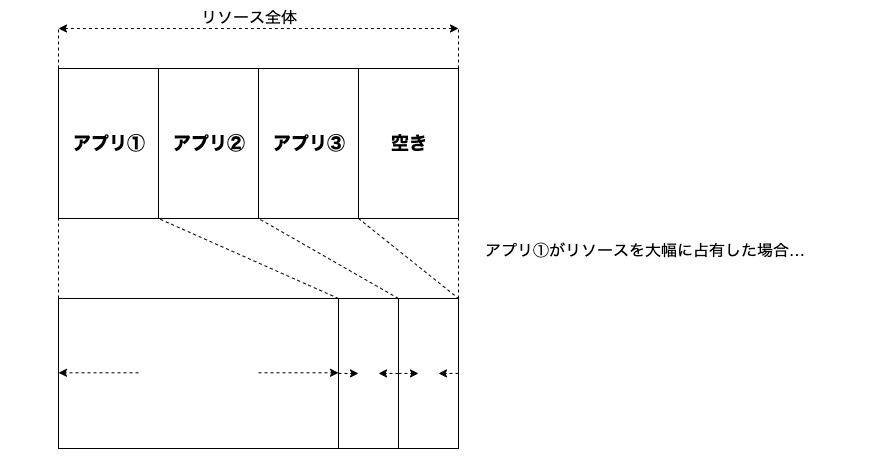
\includegraphics[width=\textwidth]{./figures/resource-on-physical-server.jpg}
    \caption{アプリケーションのひとつがリソースを大幅に占有した場合}
\end{center}
\end{figure}

解決策のひとつとして,アプリケーション毎に別々のサーバ上で動作させるものがあったが,デメリットとして維持費が嵩むことと使用されない無駄なリソースが生まれてしまうことがあった.

\begin{figure}[htbp]
\begin{center}
    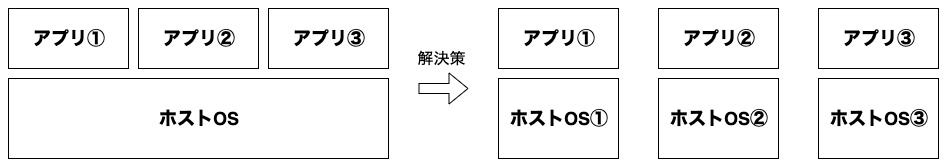
\includegraphics[width=\textwidth]{./figures/only-on-physical-server.jpg}
    \caption{ひとつの物理サーバでひとつのアプリケーションを動作させる解決策}
\end{center}
\end{figure}

これを解決するために開発されたのがVMである.
VMはソフトウェアによって仮想的に物理マシンを実現する技術であり,ひとつの物理マシンCPU上で複数のVMを動作させることが可能である.
アプリケーションはそれぞれ独立しておりお互いに不可侵な関係性であるため,ひとつのアプリケーションがリソースを占有することはなく,よりリソースを効率的に使用できる.
スケーラビリティにも長けており,開発者はいつでもアプリを追加・削除でき,ハードウェアコストの削減にも貢献している.
しかし,VMは処理におけるオーバーヘッドが大きく起動時間が長いなどデメリットも存在する.

\begin{figure}[htbp]
\begin{center}
    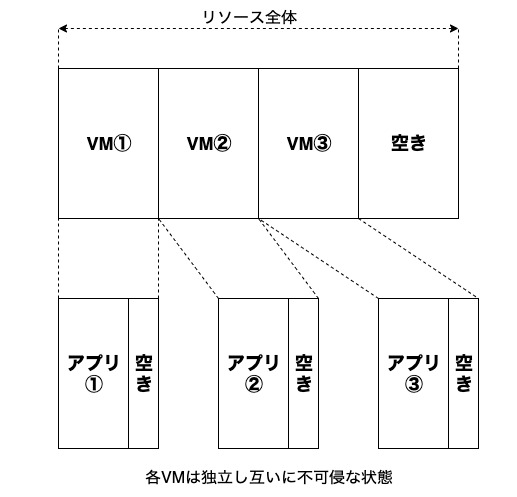
\includegraphics[width=0.8\textwidth]{./figures/resource-on-vm.jpg}
    \caption{VMの相互独立性}
\end{center}
\end{figure}

\begin{figure}[htbp]
\begin{center}
    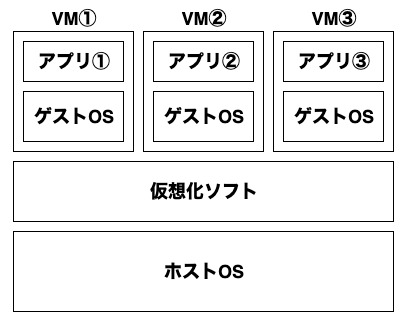
\includegraphics[width=0.6\textwidth]{./figures/vm-structure.jpg}
    \caption{VMの構成}
\end{center}
\end{figure}

VMの後に登場した技術がコンテナ型仮想化である.
コンテナ型仮想化では,各アプリケーションはひとつのホストOSを共有するため,VMより軽量で起動時間も短い.
コンテナはコンテナイメージから作成され,イメージは宣言的なファイルに基づいて生成される.
これによって開発者はより簡単かつスピーディに開発を進めることが可能である.
"Build Once, Run Anywhere"というコンセプトが掲げられており,一度生成されたイメージはどの環境でも動作し冪等性が担保される.
一方,ホストOSを共有するためセキュリティ面では課題が見られる.

\begin{figure}[htbp]
\begin{center}
    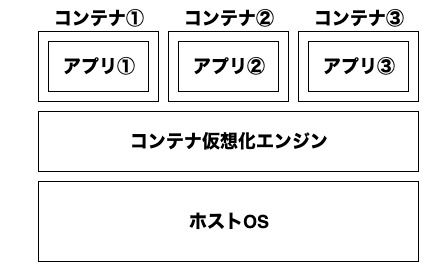
\includegraphics[width=0.6\textwidth]{./figures/docker-structure.jpg}
    \caption{コンテナ型仮想化}
\end{center}
\end{figure}

コンテナ仮想環境を構築するためのランタイムであるCRIには,dockershim(Docker), containerd, cri-o, Frakti, rktlet(rkt)などが挙げられる.
本研究では,CRIのデファクトスタンダードであるDockerを採用している.

\subsubsection{Docker}
\label{background:container-orchestration-system:container:docker}

Docker~\cite{Docker}はコンテナ型仮想環境を実現するためのプラットフォームおよびツールである.
前述したようにDockerでは,宣言的なファイルから生成したコンテナイメージを元にコンテナを起動する.
設計書となる宣言的なファイルはDockerファイルと呼ばれる.
Dockerファイルでは,ベースとなるイメージをインポートしたり,特定のコマンドの実行やファイルのコピーを行うためのコマンドが提供されている.
ミドルウェアや各種環境設定をコード化して管理することができ(Infrastructure as Code),別の環境で何度実行しても同じ結果が保証される.
Dockerイメージをバージョン毎に管理するためのDocker Hubというサービスがあり,開発者は自身のレポジトリにイメージをプッシュしたり,他のレポジトリからイメージを取得することも可能である.

\begin{figure}[htbp]
\begin{center}
    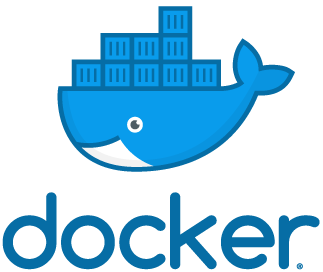
\includegraphics[width=0.4\textwidth]{./figures/docker-logo.png}
    \caption{Dockerのロゴ}
\end{center}
\end{figure}

\begin{figure}[htbp]
\begin{center}
    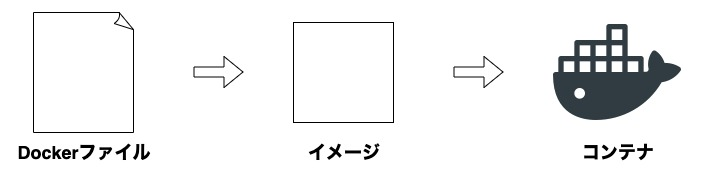
\includegraphics[width=0.8\textwidth]{./figures/docker-process.jpg}
    \caption{Dockerでのコンテナ作成手順}
\end{center}
\end{figure}

\subsection{Kubernetes}
\label{background:container-orchestration-system:kubernetes}

Kubernetes~\cite{Kubernetes}はコンテナオーケストレーションエンジンであり,コンテナ化されたアプリケーションのデプロイやスケーリングなどの管理を自動化するためのプラットフォームである.

\begin{figure}[htbp]
\begin{center}
    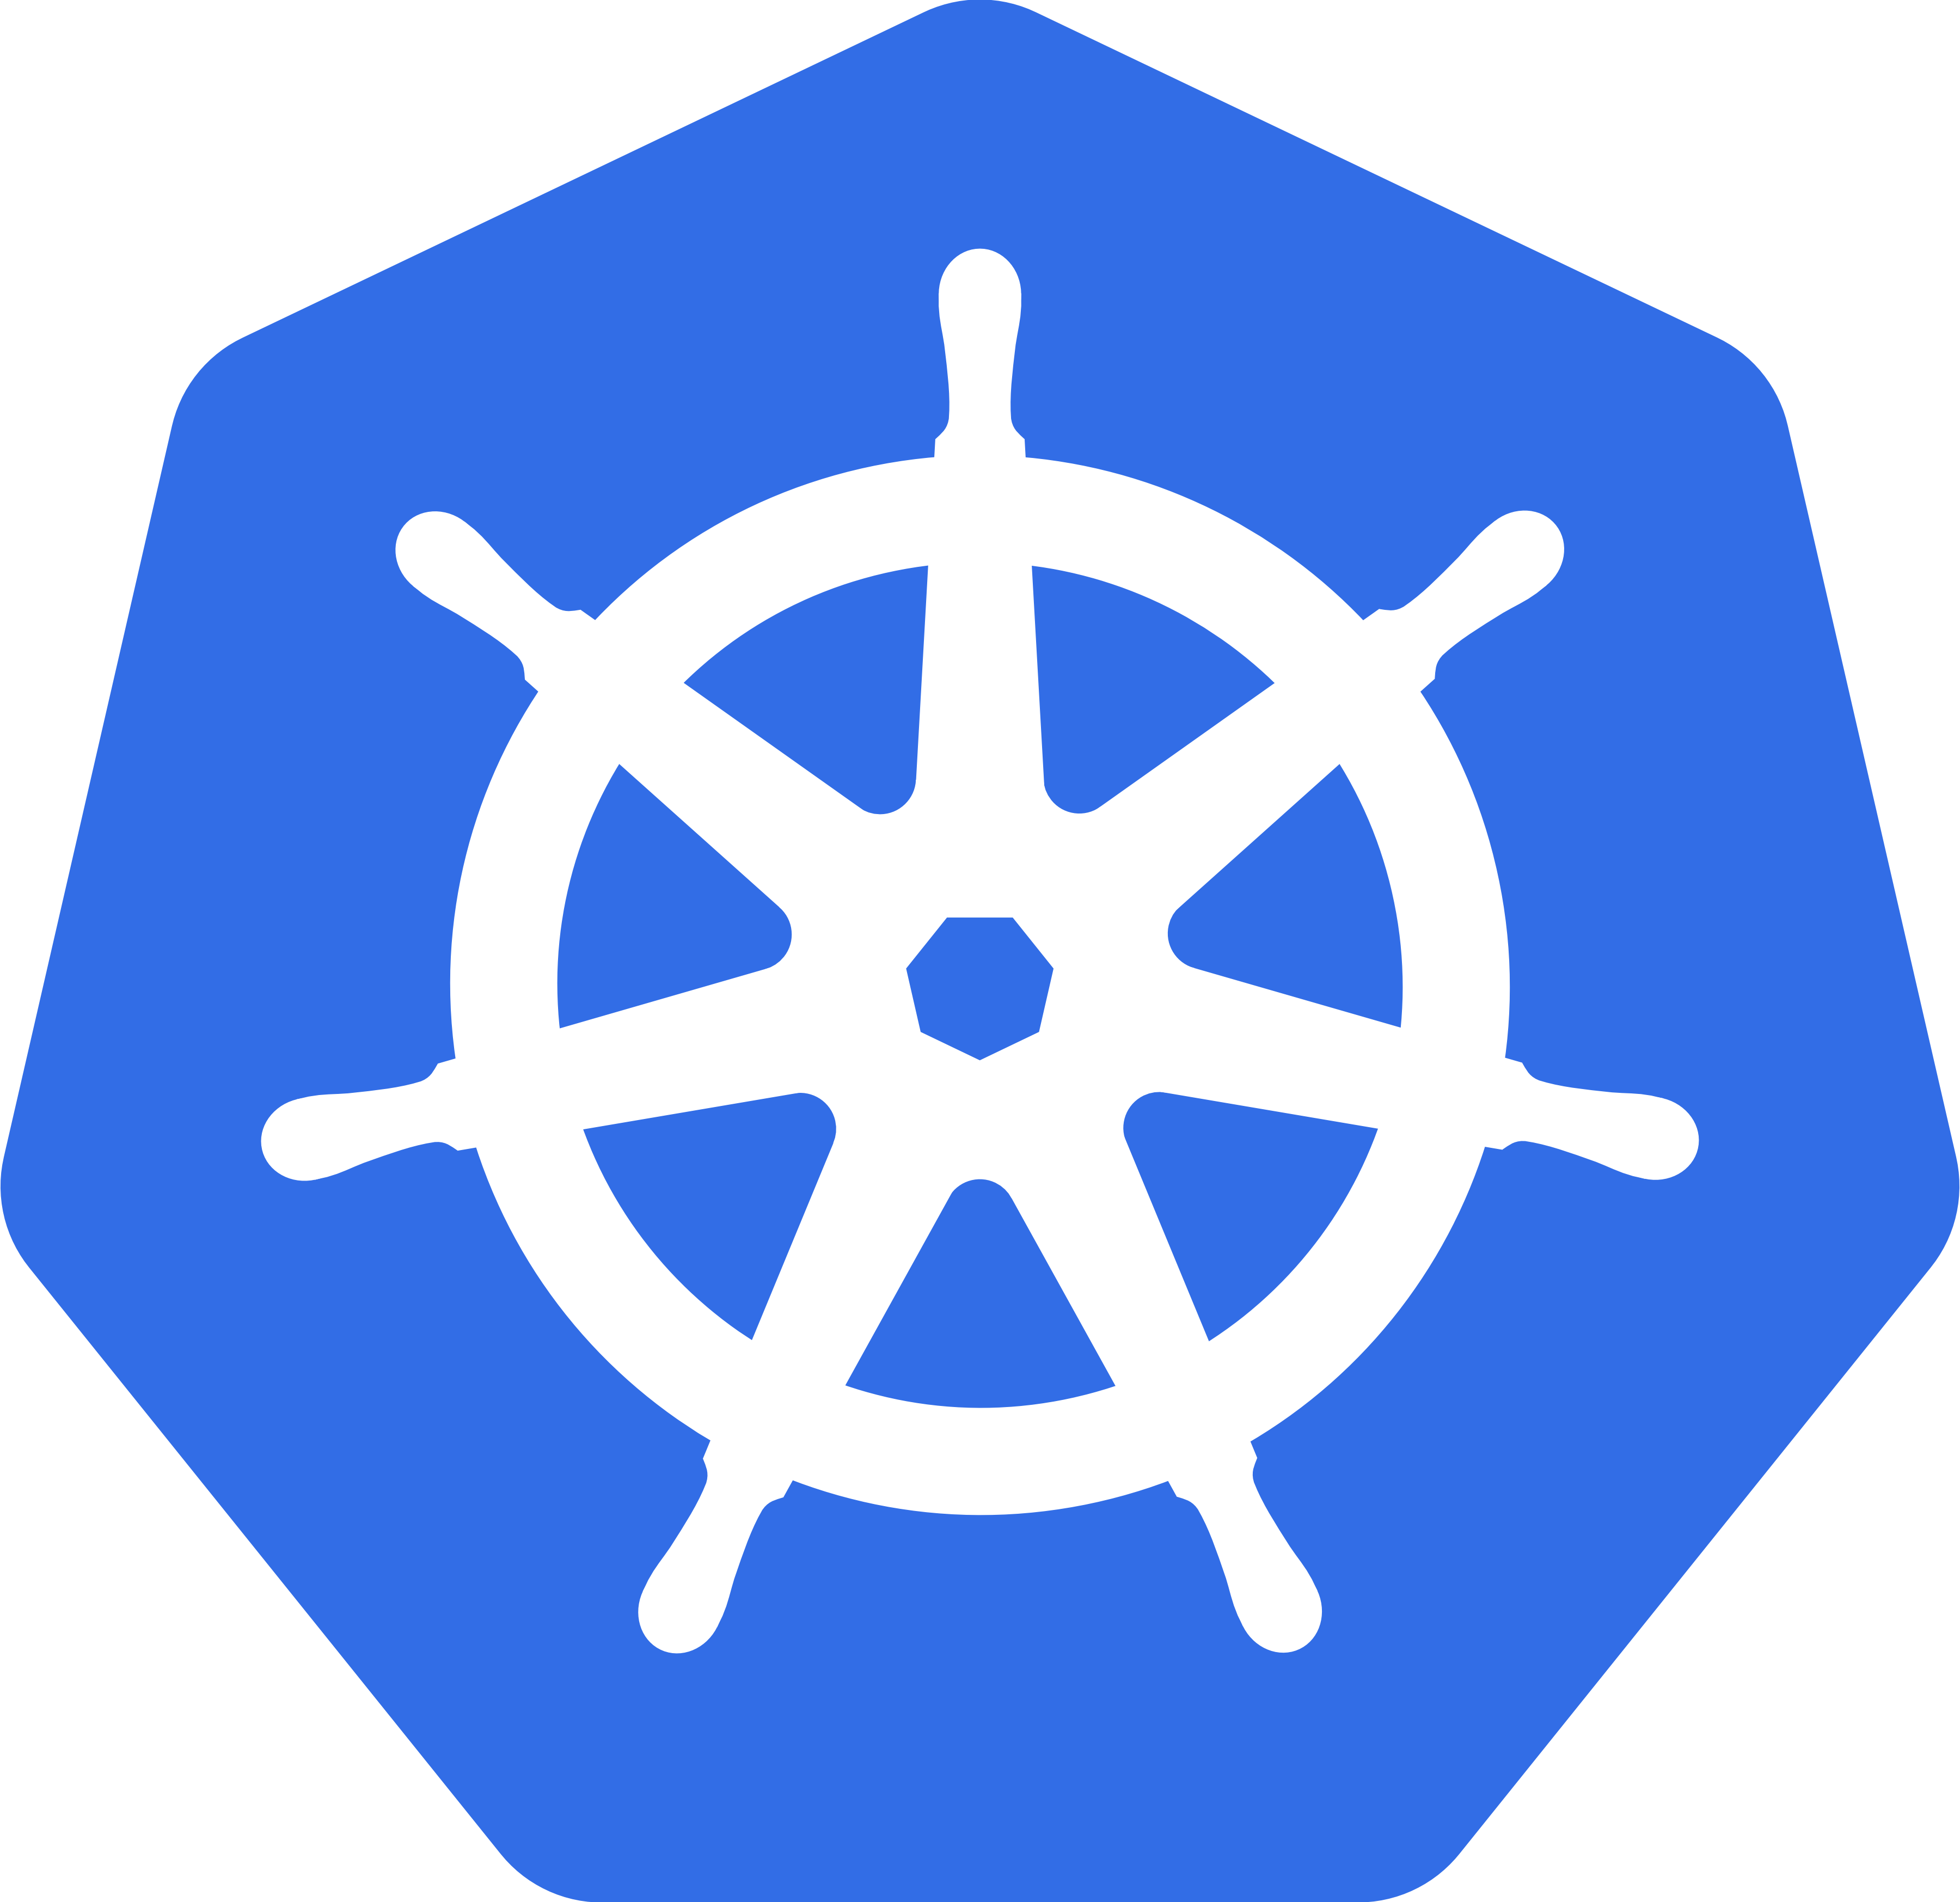
\includegraphics[width=0.4\textwidth]{./figures/kubernetes_logo.png}
    \caption{Kubernetesのロゴ}
\end{center}
\end{figure}

もともとGoogle社内で利用されていたコンテナクラスタマネージャの「Borg」を基盤にして作られたオープンソースソフトウェアであるため信頼性が高く,現時点でコンテナオーケストレーションシステムのデファクトスタンダードとなっている.
Kubernetesでは,複数のKubernetes Nodeの管理やコンテナのローリングアップデート,オートスケーリング,死活監視,ログ管理などサービスを実稼働環境で動かす上で必要不可欠となる機能を備えている.
Docker同様,デプロイするコンテナとその周辺のリソースはYAML形式やJSON形式で記述した宣言的なコードによって管理する.
Infrastructure as Codeに則っているため,実行環境に左右されず毎回常に同じコンテナが起動される.

GCPを筆頭にクラウド環境でもサポートされるようになり,現時点でAWSとAzureにおいても提供されている.
そのためKubernetesは徐々に注目を集めるようになり,今では多くの企業の実稼働環境で取り入れられている.

Kubernetesは,複数のサーバを束ねたクラスタの上で動作する.
サーバの役割は二つに分かれており,システム全体を統合管理するサーバをマスターノード(コントロールプレーン),実際にコンテナを起動させるサーバをワーカーノードと呼ぶ.
マスターノードはシングルでも動作するが,基本的には冗長性や耐障害性を考慮して複数のマスターノードをクラスタリングすることが多い.
クラウド環境を用いた場合,クリックひとつでKubernetesクラスタを用意することができる.
状況に応じてワーカーノードを追加・削除でき,自由にスケーリング出来る点も強みである.
クラウドの種類によっては特定の条件に合わせて自動でノードのオートスケーリングを行うこともできるが,オンプレ環境では自前で実装する必要がある.

\begin{figure}[htbp]
\begin{center}
    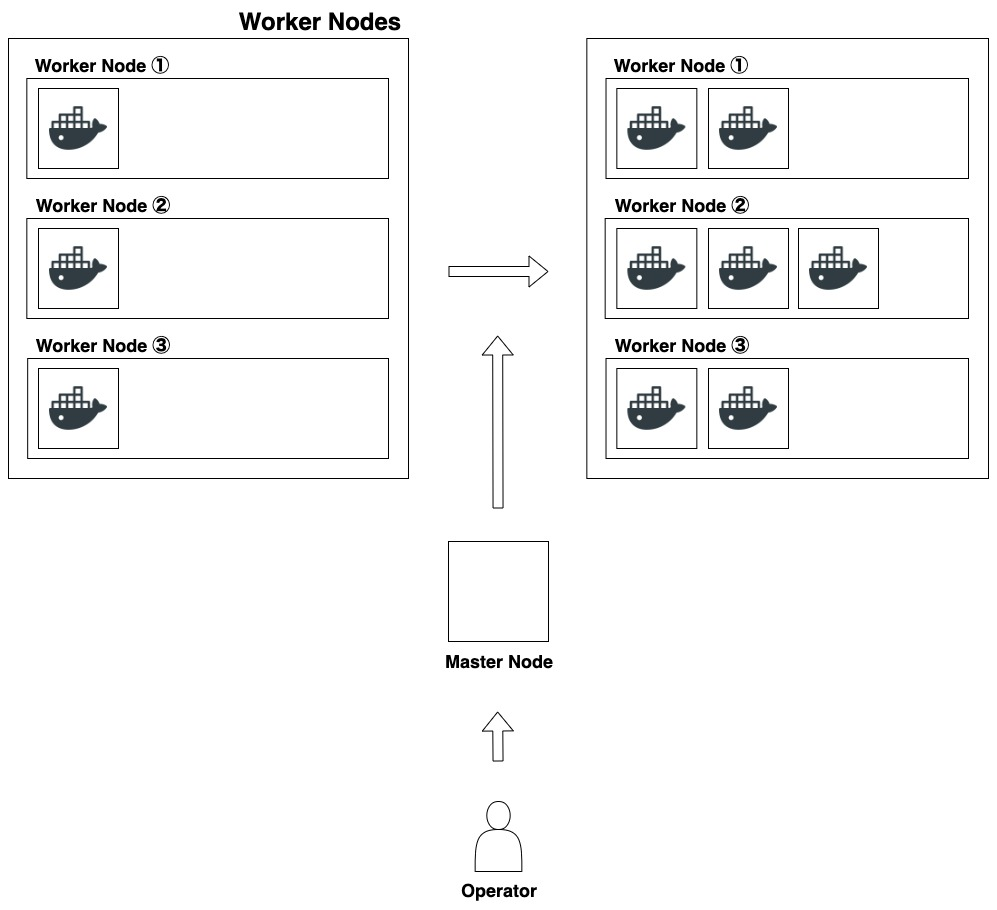
\includegraphics[width=\textwidth]{./figures/k8s-deploy-container.jpg}
    \caption{Kubernetesでのコンテナデプロイ}
\end{center}
\end{figure}

Kubernetes自体は,多数のコンポーネントによって構成されるマイクロサービスアーキテクチャを採用している.
すべてのコンポーネントがkube-apiserverと呼ばれるKubernetes内のAPIサーバを中心として動作しており,殆ど全ての処理はkube-apiserverを通して実行される.
kube-apiserverはマスターノードに含まれる.
他にもマスターノード内で動作するコンポーネントとしては,
Kubernetesクラスタのすべての情報を保持するetcd,
コンテナを起動させるノードをスケジューリングするkube-scheduler,
ノード上で動作するコンテナを監視し必要に応じてコンテナを追加・削除するよう指示するkube-controller-managerなどが挙げられる.
対してワーカーノードで動作する主なコンポーネントには,kubeletなどがある.
kubeletを含め,本研究の実装で用いたkubeadm,kubectlに関しては以下で詳細に説明する.

\subsubsection{Kubeadm}
\label{background:container-orchestration-system:kubernetes:kubeadm}

Kubeadm~\cite{Kubeadm}は,Kubenetesクラスタを構築するためのベストプラクティスを提供するツールである.
Kubeadmが提供するコマンドをいくつか以下に示す.\\*

{\bf kubeadm init}\\
クラスタの最初のコントロールプレーンとなるノードを起動する.\\*

{\bf kubeadm join}\\
クラスタに追加のコントロールプレーンまたはワーカーノードを参加させる.\\*

{\bf kubeadm upgrade}\\
クラスタのバージョンを最新へアップグレードする.\\*

{\bf kubeadm reset}\\
kubeadm initやkubeadm joinによって生じた変更を取り消す.\\*

\subsubsection{kubelet}
\label{background:container-orchestration-system:kubernetes:kubelet}

kubelet~\cite{kubelet}は,Kubernetesクラスタ内の各ワーカーノードで動作するコンポーネントである.
kubectlは,DockerなどのCRIと連携して実際にコンテナを起動・停止する役割をもつ.
具体的にはetcdの情報を監視して,自身のノードに割り当てられてまだ起動していないコンテナがあれば起動する.
etcdに格納された情報は,kube-apiserverやkube-controller-managerによってkube-apiserverを通して書き換えられ,実際のコンテナの操作に関してはkubeletが担うといった役割分担がされている.
~\ref{background:container-orchestration-system:kubernetes:kubeadm}章のkubeadm,ならびに~\ref{background:container-orchestration-system:kubernetes:kubectl}章のkubectlは,Kubernetesクラスタ構築時や操作時に用いるコマンドツールであるのに対して,
kubeletはコンテナの管理を行うデーモンとして動作する.

\subsubsection{kubectl}
\label{background:container-orchestration-system:kubernetes:kubectl}

kubectl~\cite{kubectl}は,Kubernetesクラスタをコントロールするためのツールである.
新規コンテナのデプロイや削除,アップデートから,動作中のコンテナやクラスタを構成するノードの情報の取得など,サービスの
運用を支援するAPIが提供されている.
kubectlが提供するコマンドをいくつか以下に示す.\\*

{\bf kubectl get nodes}\\
クラスタに参加するノードのステータスやロール(役割),IPアドレス等を取得する.\\*

{\bf kubectl get pods}\\
ポッドの名前やステータス,再起動の回数等を取得する.\\*

{\bf kubectl apply}\\
ポッドに新たな設定を反映させる.\\*

\section{OpenVPN}
\label{background:openvpn}

本節では,本研究で使用したVPN技術ならびにソフトウェアVPNであるOpenVPNについて概説する.

VPNとは,``Virtual Private Network''の略で,日本語では``仮想専用線''と呼ばれる.
VPNは,インターネット上に擬似的なプライベートネットワークを実現する技術,またはそのネットワーク自体を指す.
VPNを使用することで,インターネット上の異なるセグメント同士であっても,あたかも専用線で接続されているかのように通信することが可能である.
VPNにはL2VPNとL3VPNがあり,L2VPNは異なるセグメント同士を接続しひとつの擬似的なLANを構築するものであり,L3VPNではIPプロトコルでの通信が可能となる.
セキュリティ面においては,通信内容をカプセル化することでパケットの中身の覗き見や改竄のリスクを低減することができる.

\begin{figure}[htbp]
\begin{center}
    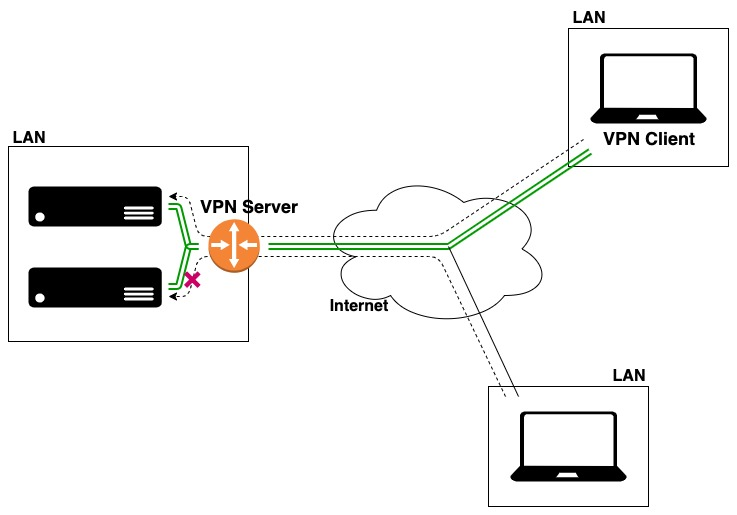
\includegraphics[width=0.8\textwidth]{./figures/openvpn.jpg}
    \caption{VPN}
\end{center}
\end{figure}

\subsection{OpenVPN}

OpenVPN~\cite{OpenVPN}は,OpenVPN Technologies, inc.が中心になって開発しているオープンソースのVPNソフトウェアである.

\begin{figure}[htbp]
\begin{center}
    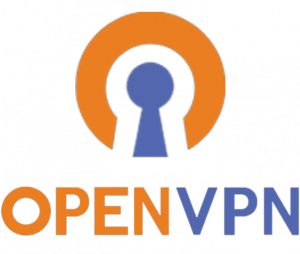
\includegraphics[width=0.4\textwidth]{./figures/openvpn-logo.png}
    \caption{OpenVPNのロゴ}
\end{center}
\end{figure}

OpenVPNは幅広いOSでサポートされており,Window, Linux, Mac OS, iOS, Androidで利用可能である.
異なるOS間でも利用可能であるため,ひとつのVPNネットワーク内に異なるOSが混在していても正常に動作する.
OpenVPNでは,対応したOSのサーバがひとつでもあれば簡単にVPNサーバを構築することが可能である.
VPNネットワークに参加するためには認証が必要であり,OpenVPNでは静的鍵による認証や証明書認証,ID/パスワード認証,二要素認証といった複数の認証方法から任意のものを選択できる.
接続方法としては,ルーティングとブリッジが提供され,ルーティングはL3VPN, ブリッジはL2VPNに対応する.
VPNネットワーク内でブロードキャストを行いたい場合など,擬似的なLANを構築したい場合以外は基本的にL3VPNを用いる.
L3VPNにあたるルーティングでは,クライアントサーバ接続とサイト間接続が提供されている.
クライアントサーバ接続では,各クライアントに認証設定が必要となり,接続の準備としてサーバ側での認証情報の生成が必要となる.
認証情報を共有後,クライアント側では接続のために設定ファイルを用意し,コマンドやアプリケーションを用いて接続を行う.
対するサイト間接続では,VPNの設定は各セグメントのVPNサーバで完結する.
VPNサーバ間での接続が確立できれば,各拠点に配置されたサーバはお互いに疎通が可能となる.
本研究の提案手法においては,ルーティング形式のサイト間接続を活用した.
